\documentclass[conference]{IEEEtran}
\IEEEoverridecommandlockouts
% The preceding line is only needed to identify funding in the first footnote. If that is unneeded, please comment it out.
\usepackage{cite}
\usepackage{amsmath,amssymb,amsfonts}
\usepackage{algorithmic}
\usepackage{graphicx}
\usepackage{textcomp}
\usepackage{xcolor}
\def\BibTeX{{\rm B\kern-.05em{\sc i\kern-.025em b}\kern-.08em
    T\kern-.1667em\lower.7ex\hbox{E}\kern-.125emX}}
\begin{document}

\title{Real-Time Power Quality Disturbance Classification Using Hyperparameter-Tuned Random Forest with Multi-Domain Feature Extraction for Edge Deployment\\
}

\author{
\begin{minipage}{0.32\textwidth}
\centering
\textbf{Shrimathi G} \\
\textit{Department of Electrical and Electronics Engineering} \\
\textit{Sri Venkateswara College of Engineering} \\
Pennalur 602117 \\
2022ee0135@svce.ac.in
\end{minipage}
\hfill
\begin{minipage}{0.32\textwidth}
\centering
\textbf{Sanjay Kumar V} \\
\textit{Department of Electrical and Electronics Engineering} \\
\textit{Sri Venkateswara College of Engineering} \\
Pennalur 602117 \\
2022ee0214@svce.ac.in
\end{minipage}
\hfill
\begin{minipage}{0.32\textwidth}
\centering
\textbf{Suresh N} \\
\textit{Department of Electrical and Electronics Engineering} \\
\textit{Sri Venkateswara College of Engineering} \\
Pennalur 602117 \\
sureshn@svce.ac.in
\end{minipage}
}
\maketitle

\begin{abstract}
This paper presents a hyperparameter-tuned Random Forest classifier for automatic classification of 17 power quality disturbance types defined under IEEE 1159, including eight compound disturbance classes. Thirty-six features are extracted from raw voltage signals across three domains: 14 time-domain features including root mean square, peak, kurtosis, and crest factor; 10 frequency-domain features including total harmonic distortion and harmonic magnitudes; and 12 wavelet-domain features derived from three-level Daubechies-4 decomposition. The XPQRS dataset comprising 17,000 signals of 100 samples each at 5000 Hz is used for training and evaluation with an 80 to 20 stratified split. Hyperparameter optimization using Randomized Search with 5-fold cross-validation yields 200 decision trees with logarithmic feature selection. The proposed classifier achieves a classification accuracy exceeding 95 percent at an inference time below 100 milliseconds, without requiring GPU hardware or cloud infrastructure, demonstrating suitability for real-time edge-compatible power quality monitoring.
\end{abstract}

\begin{IEEEkeywords}
Power Quality, Power Quality Disturbances (PQD), Random Forest, Machine Learning, Feature Extraction, Signal Processing, Wavelet Transform, Harmonics, Voltage Sag, Voltage Swell, Real-Time Monitoring, Edge Computing
\end{IEEEkeywords}

\section{Introduction}
Power quality (PQ) has become a significant concern in modern power systems due to the increasing integration of renewable energy sources, nonlinear loads, and power electronic devices. Disturbances such as voltage sag, swell, harmonics, flicker, and transient events adversely affect system stability, energy efficiency, and the lifespan of electrical equipment. Recent studies highlight that a major portion of power system disturbances originates from such PQ issues, emphasizing the need for accurate and real-time monitoring systems \cite{b1}, \cite{b7}.

Traditional signal processing techniques, such as Fast Fourier Transform (FFT) and Root Mean Square (RMS) analysis, have been widely used for detecting PQ disturbances. However, these methods are limited in their ability to capture non-stationary, transient, and complex disturbances in dynamic power systems \cite{b8}. As modern grids become more complex with the integration of distributed energy resources, conventional approaches struggle to provide reliable and timely classification.

To address these limitations, machine learning (ML) and deep learning (DL) techniques have been extensively applied to PQ disturbance classification. Methods such as Extreme Learning Machines (ELM) \cite{b3}, wavelet-based feature extraction combined with ML models \cite{b6}, and hybrid deep learning approaches \cite{b4} have demonstrated high classification accuracy. Additionally, advanced architectures such as Convolutional Neural Networks and Vision Transformers have achieved near-perfect performance; however, they require high computational resources and complex preprocessing, limiting their suitability for real-time applications \cite{b10}.

Among various ML techniques, ensemble learning methods such as Random Forest (RF) have gained significant attention due to their robustness, interpretability, and ability to handle high-dimensional data. Previous studies have shown that RF can achieve competitive accuracy while maintaining lower computational complexity compared to deep learning models \cite{b2}, \cite{b5}. Furthermore, feature extraction techniques incorporating time-domain, frequency-domain, and wavelet-domain characteristics have been proven effective in improving classification performance \cite{b9}.

Despite these advancements, existing solutions still face challenges related to computational cost, latency, and real-time deployment. Many approaches rely on cloud-based processing or high-performance hardware, making them impractical for edge-based implementations. Moreover, achieving an optimal balance between accuracy, speed, and scalability remains an open research problem.

In this paper, a machine learning-based approach for power quality disturbance classification using the Random Forest algorithm is proposed. The system focuses on achieving high classification accuracy with low inference time, making it suitable for real-time and edge-based applications. The proposed model utilizes multi-domain feature extraction techniques and is designed to provide reliable and efficient classification of various PQ disturbances. The results demonstrate the effectiveness of the proposed approach in improving performance while maintaining computational efficiency. 

\section{Literature Review}

Power quality disturbance (PQD) detection and classification have been widely studied using both traditional signal processing and intelligent techniques. A comprehensive review presented in \cite{b1} summarizes various methods including Fourier-based, wavelet-based, and machine learning approaches. The study highlights that conventional techniques are limited in handling non-stationary and transient disturbances, thereby motivating the adoption of intelligent models.

In \cite{b2}, an adaptive boosted Random Forest approach combined with optimization techniques is proposed for PQD classification. The method demonstrates improved accuracy and robustness by enhancing feature selection and model performance. Similarly, a comparative study in \cite{b5} evaluates multiple machine learning algorithms for PQD classification and concludes that ensemble methods such as Random Forest provide competitive accuracy while maintaining computational efficiency.

Extreme Learning Machine (ELM) has also been applied for PQD classification. In \cite{b3}, an identity feature vector-based ELM model is used to classify multiple disturbance types, achieving high accuracy for most classes. However, its performance decreases for complex combined disturbances, indicating limitations in generalization.

Feature extraction techniques play a significant role in improving classification performance. In \cite{b6}, a dual-stage approach combining discrete wavelet transform (DWT) with ELM is proposed, showing effective detection of transient disturbances. Similarly, \cite{b9} presents a wavelet packet-based energy feature extraction method that enhances the detection of voltage sag and other disturbances. Furthermore, \cite{b8} analyzes various signal processing techniques including FFT, STFT, CWT, and DWT, and concludes that wavelet-based methods outperform traditional Fourier techniques in handling non-stationary signals.

Deep learning approaches have also been explored for PQD classification. In \cite{b4}, a hybrid deep learning model is proposed for disturbance identification in renewable energy systems, achieving high classification accuracy. In addition, \cite{b10} compares Vision Transformers and Convolutional Neural Networks for PQD classification, demonstrating near-perfect accuracy. However, these models require high computational resources, complex preprocessing, and are less suitable for real-time deployment.

From the above studies, it is evident that while deep learning models provide high accuracy, they are computationally intensive. Traditional methods lack the capability to handle complex disturbances effectively. Machine learning approaches, particularly ensemble methods, offer a balance between accuracy and efficiency. Therefore, there is a need for a computationally efficient and accurate model that can be deployed in real-time environments, which motivates the proposed Random Forest-based approach.
\section{Problem Statement and Contributions}

\subsection{Problem Statement}

Modern power systems are increasingly affected by power quality disturbances due to the widespread integration of renewable energy sources, power electronic converters, and nonlinear loads. These disturbances, including voltage sag, swell, harmonics, and transient events, introduce non-stationary and nonlinear characteristics in voltage signals, making their detection and classification a challenging task.

Conventional signal processing techniques such as Fast Fourier Transform (FFT) and Root Mean Square (RMS) analysis are effective for steady-state conditions but are limited in capturing transient and time-varying disturbances. These methods often fail to provide accurate classification in complex scenarios involving overlapping or compound disturbances.

Recent advancements in machine learning and deep learning have improved classification performance. However, many deep learning-based approaches require high computational resources, large training datasets, and complex preprocessing, which restrict their applicability in real-time and edge-based environments. Additionally, some machine learning models lack interpretability, making it difficult to understand the contribution of individual features to the classification outcome.

Therefore, there exists a need for a classification framework that can accurately identify multiple types of power quality disturbances while maintaining low computational complexity, real-time capability, and model interpretability.

\subsection{Contributions}

To address the above challenges, this work presents a machine learning-based framework for power quality disturbance classification with the following key contributions:

\begin{itemize}
\item A Random Forest-based classification model is developed to accurately identify multiple power quality disturbances, leveraging its ensemble structure for improved generalization and robustness.

\item A multi-domain feature extraction approach is implemented, incorporating time-domain, frequency-domain, and wavelet-domain features to capture both steady-state and transient characteristics of the signal.

\item A computationally efficient pipeline is designed with low inference latency, making the proposed system suitable for real-time and edge-based deployment.

\item SHAP-based explainability is integrated to analyze feature contributions, improving model transparency and enabling better understanding of the classification decisions.

\item The proposed method achieves a balance between classification accuracy and computational efficiency, addressing the limitations of both traditional signal processing and deep learning approaches.
\end{itemize}

\section{Methodology}

\subsection{System Overview}

The proposed framework is designed for the classification of power quality disturbances (PQDs) using a machine learning-based approach. The system follows a structured pipeline consisting of signal acquisition, preprocessing, feature extraction, model training, and classification. The objective is to achieve high classification accuracy with low computational complexity, enabling real-time deployment.

\subsection{System Architecture}

The overall architecture of the proposed system is illustrated in Fig.~\ref{fig:architecture}. The framework consists of sequential processing stages starting from signal acquisition to final classification output.

\begin{figure}[h]
    \centering
    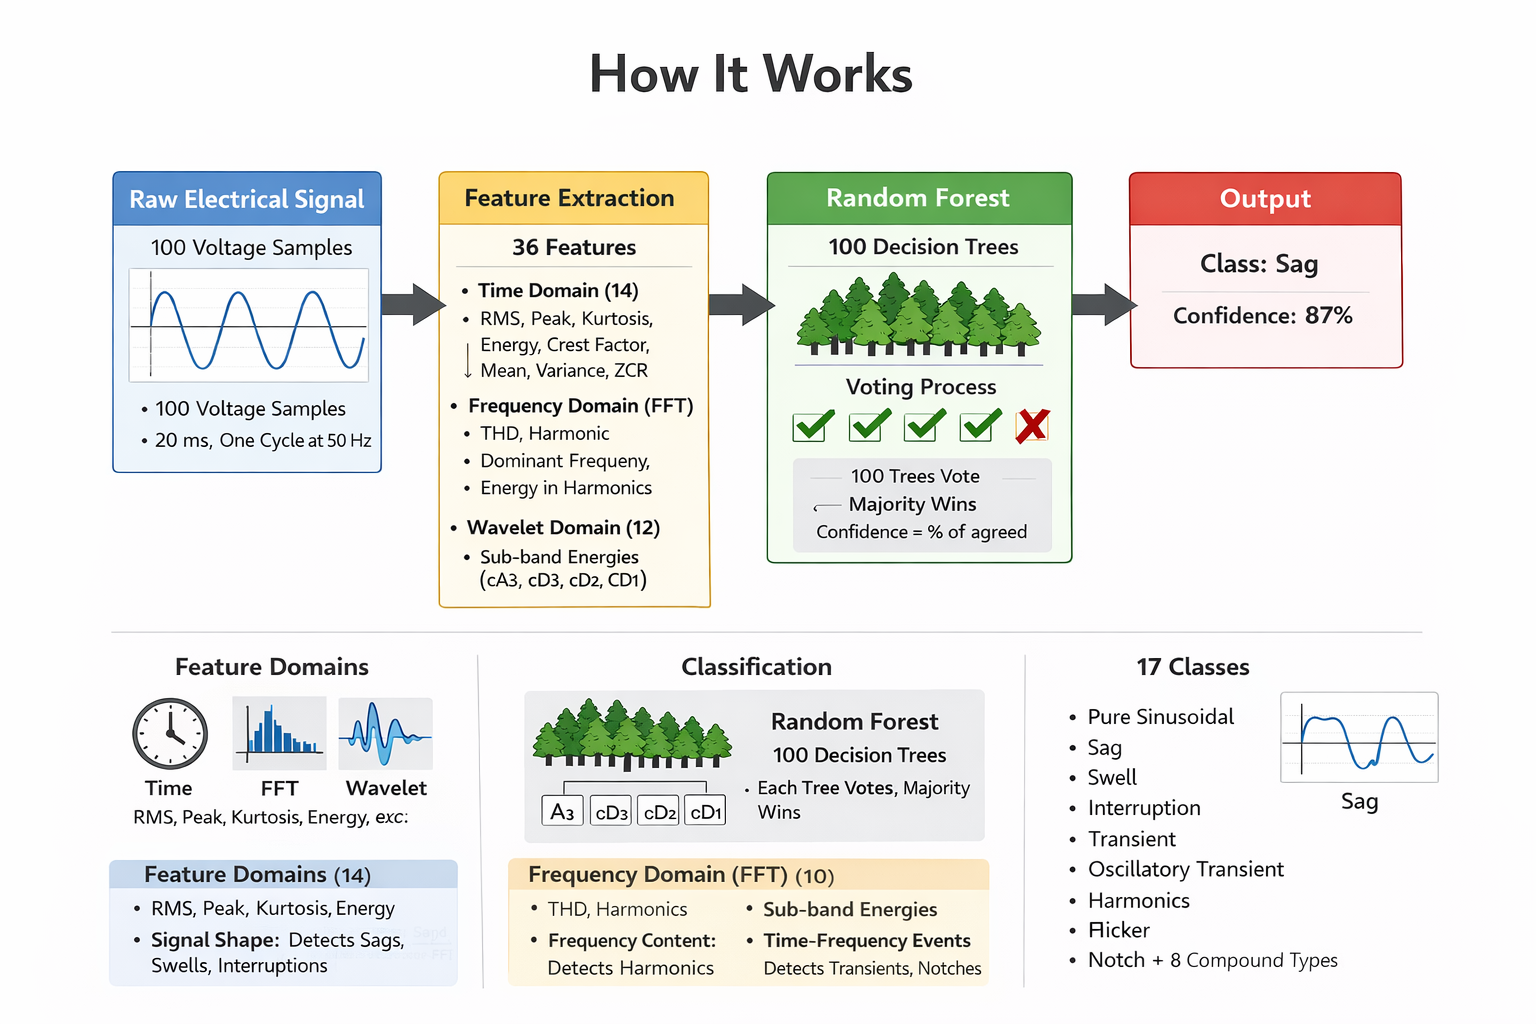
\includegraphics[width=0.75\linewidth]{image.png}
    \caption{Power quality disturbance classification system showing signal acquisition, multi-domain feature extraction, Random Forest-based classification, and output prediction}
    \label{fig:architecture}
\end{figure}

Initially, voltage signals are obtained from the power system and passed through a preprocessing stage to remove noise and normalize the data. The processed signals are then subjected to multi-domain feature extraction, where time-domain, frequency-domain, and wavelet-domain features are computed.

The extracted feature vector is provided as input to the Random Forest classifier. The model processes the input features and outputs the predicted disturbance class. The modular structure of the system ensures efficient implementation and supports real-time operation.


\subsection{Signal Acquisition and Preprocessing}

The input to the system consists of discrete-time voltage signals representing different PQ disturbances such as sag, swell, harmonics, and flicker. Each signal is represented as:

\begin{equation}
x(n), \quad n = 1,2,3,...,N
\end{equation}

where $N$ denotes the number of samples.

Preprocessing is performed to improve signal quality and ensure consistency. The signal is normalized as:

\begin{equation}
\tilde{x}(n) = \frac{x(n) - \mu}{\sigma}
\end{equation}

where $\mu$ and $\sigma$ represent the mean and standard deviation of the signal. This step removes scaling variations and improves model performance.

\subsection{Feature Extraction}

Feature extraction transforms raw signals into informative representations. To capture both steady-state and transient characteristics, features are extracted from multiple domains.

\subsubsection{Time-Domain Features}

Time-domain features include statistical measures such as RMS, mean, and crest factor.

\begin{equation}
V_{\text{RMS}} = \sqrt{\frac{1}{N} \sum_{i=1}^{N} x_i^2}
\end{equation}

\begin{equation}
\mu = \frac{1}{N} \sum_{i=1}^{N} x_i
\end{equation}

\begin{equation}
CF = \frac{V_{\text{peak}}}{V_{\text{RMS}}}
\end{equation}

These features describe amplitude and distribution characteristics of the signal.

\subsubsection{Frequency-Domain Features}

Frequency-domain features are obtained using the Fast Fourier Transform (FFT). The Total Harmonic Distortion (THD) is computed as:

\begin{equation}
THD = \frac{\sqrt{\sum_{n=2}^{H} V_n^2}}{V_1}
\end{equation}

where $V_n$ is the magnitude of the $n^{th}$ harmonic and $V_1$ is the fundamental component.

\subsubsection{Wavelet-Domain Features}

Discrete Wavelet Transform (DWT) is used to capture transient characteristics. The energy of wavelet coefficients at each level is given by:

\begin{equation}
E_j = \sum_{k=1}^{M} |d_{j,k}|^2
\end{equation}

These features are effective in identifying non-stationary disturbances.

\subsection{Feature Normalization}

The extracted feature vectors are standardized to ensure uniform scaling. This prevents features with large magnitudes from dominating the model and improves convergence.

\subsection{Model Development}

A Random Forest classifier is employed for PQD classification. The model consists of multiple decision trees trained using bootstrap sampling. At each split, a random subset of features is selected to introduce diversity and reduce overfitting.

The final prediction is obtained using majority voting:

\begin{equation}
Y = \text{mode}(Y_1, Y_2, ..., Y_T)
\end{equation}

where $T$ represents the number of trees.

\subsection{Hyperparameter Optimization}

The performance of the model depends on parameters such as the number of trees, maximum depth, and minimum samples per split. These parameters are tuned using cross-validation to achieve optimal performance. Increasing the number of trees improves accuracy, while limiting depth controls overfitting.

\subsection{Computational Complexity}

The computational complexity of the Random Forest model increases with the number of trees and feature dimensions. However, since trees are independent, training can be parallelized. The inference time remains low, making the model suitable for real-time applications.

\subsection{Classification Process}

During prediction, new signals undergo the same preprocessing and feature extraction steps. The trained model processes the feature vector and outputs the predicted disturbance class.

\subsection{Real-Time Implementation Considerations}

The proposed system is designed for real-time operation with low latency. Efficient feature extraction and lightweight model architecture enable deployment on edge devices. This reduces dependency on cloud-based systems and ensures faster response in practical applications.

The practical deployment architecture of the proposed system is illustrated in Fig.~\ref{fig:implementation}.The system integrates sensing, edge processing, and monitoring components for real-time power quality disturbance analysis.

\begin{figure}[h]
    \centering
    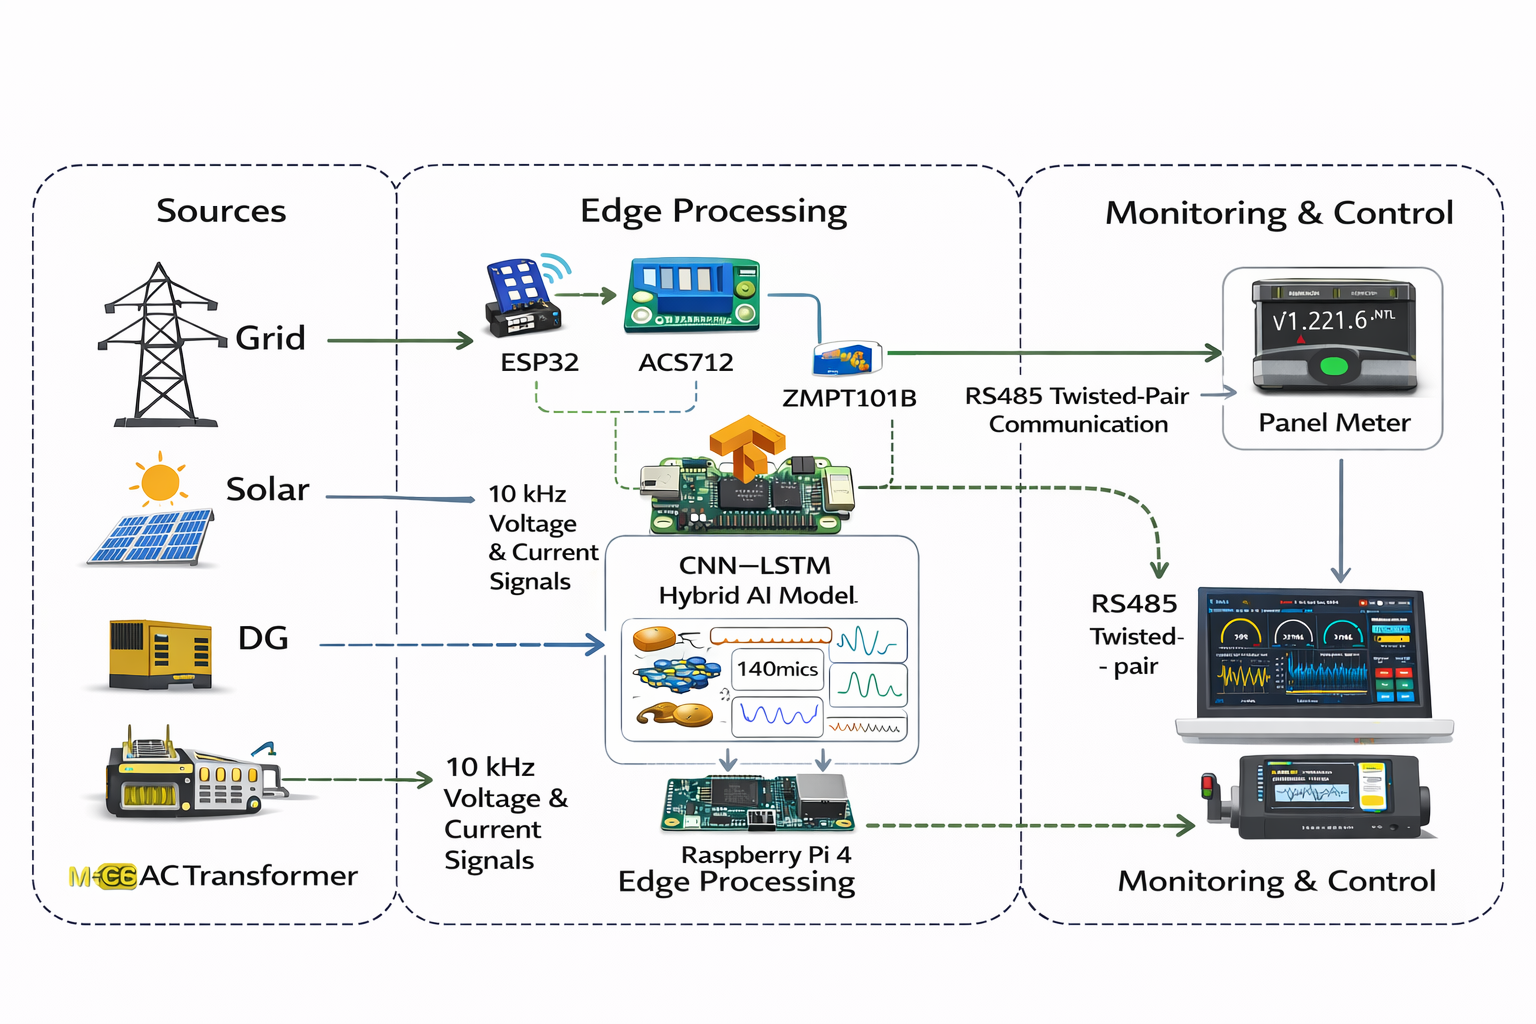
\includegraphics[width=0.75\linewidth]{image2.png}
    \caption{Practical implementation architecture of the proposed power quality disturbance monitoring system illustrating signal acquisition from multiple sources, edge-based processing, and real-time monitoring and control}
    \label{fig:implementation}
\end{figure}

The system consists of multiple stages including signal acquisition, edge processing, and monitoring. Voltage and current signals are acquired from various sources such as grid, solar, and distributed generation systems.

The acquired signals are processed using sensing modules and transmitted to an edge processing unit. Feature extraction and classification are performed at the edge using the trained machine learning model. The classification results are communicated through RS485-based communication for monitoring and control.

The modular architecture enables real-time analysis, reduces latency, and supports scalable deployment in practical power systems.

\section{Model Comparison and Selection}

To evaluate the effectiveness of different machine learning algorithms for power quality disturbance (PQD) classification, multiple models were trained and tested under identical conditions. The models considered include Logistic Regression, Support Vector Machine (SVM), k-Nearest Neighbors (kNN), Decision Tree (DT), and Random Forest (RF). All models were trained using the same feature set derived from multi-domain feature extraction to ensure a fair comparison.

The performance of these models was evaluated using two datasets, namely XPQRS and PQ datasets, with metrics such as accuracy and F1-score. The results are summarized in Table~\ref{tab:model_comparison}.
\begin{table}[h]
\centering
\caption{Performance Comparison of Models}
\label{tab:model_comparison}
\resizebox{\columnwidth}{!}{%
\begin{tabular}{|c|c|c|c|c|}
\hline
Model & XPQRS Acc & PQ Acc & XPQRS F1 & PQ F1 \\
\hline
RF & 0.9062 & 0.9812 & 0.9056 & 0.9816 \\
DT & 0.8650 & 0.9625 & 0.8646 & 0.9620 \\
LR & 0.8524 & 0.9375 & 0.8489 & 0.9372 \\
SVM & 0.8335 & 0.8812 & 0.8298 & 0.8798 \\
KNN & 0.8006 & 0.9062 & 0.7955 & 0.9046 \\
\hline
\end{tabular}%
}
\end{table}

The results indicate that Random Forest consistently achieves the highest performance across both datasets. On the XPQRS dataset, Random Forest attains an accuracy of 0.9062 and an F1-score of 0.9056, outperforming all other models. Similarly, on the PQ dataset, it achieves an accuracy of 0.9812 and an F1-score of 0.9816, demonstrating strong generalization capability.

Decision Tree exhibits competitive performance with an accuracy of 0.8650 (XPQRS) and 0.9625 (PQ), but its performance is slightly lower than Random Forest due to its tendency to overfit individual training samples. Logistic Regression and SVM show moderate performance, indicating limitations in capturing complex and non-linear relationships present in PQ disturbances. The kNN model records comparatively lower performance, which can be attributed to its sensitivity to noise and increased computational cost during inference.

The superior performance of Random Forest can be attributed to its ensemble learning mechanism, where multiple decision trees are combined to improve generalization and reduce variance. Additionally, its ability to handle high-dimensional feature spaces and noisy data makes it well-suited for PQD classification.

Based on the comparative analysis, Random Forest is selected as the optimal model for the proposed system. It provides the best balance between classification accuracy, robustness, and computational efficiency, making it suitable for real-time power quality monitoring applications.


\section{Results and Discussion}

\subsection{Experimental Setup and Hyperparameter Settings}

The Random Forest model is optimized using RandomizedSearchCV with 5-fold cross-validation to identify the most effective hyperparameter configuration. The tuning process is performed using accuracy as the evaluation metric.

The optimized hyperparameters are summarized in Table~\ref{tab:hyperparameters}.

\begin{table}[h]
\centering
\caption{Optimized Hyperparameters for Random Forest Model}
\label{tab:hyperparameters}
\begin{tabular}{|c|c|}
\hline
Hyperparameter & Value \\
\hline
Number of Trees ($n_{\text{estimators}}$) & 200 \\
Minimum Samples Split ($min\_samples\_split$) & 2 \\
Minimum Samples Leaf ($min\_samples\_leaf$) & 1 \\
Maximum Features ($max\_features$) & $\log_2$ \\
Maximum Depth ($max\_depth$) & None \\
Class Weight ($class\_weight$) & None \\
\hline
\end{tabular}
\end{table}

The selection of 200 trees improves model stability and reduces variance. The minimum split and leaf parameters allow the model to capture fine-grained patterns in PQ signals. The use of $\log_2$ features introduces randomness at each split, improving generalization. The depth of the trees is not restricted, while overfitting is controlled through ensemble learning.

\subsection{Performance Evaluation}

The performance of the proposed system is evaluated using accuracy and F1-score as primary metrics. A detailed comparison of different machine learning models is presented in Section~\ref{tab:model_comparison}, where the Random Forest model demonstrates superior performance across both XPQRS and PQ datasets.

\subsection{Prediction Output Analysis}

\begin{figure}[h]
    \centering
    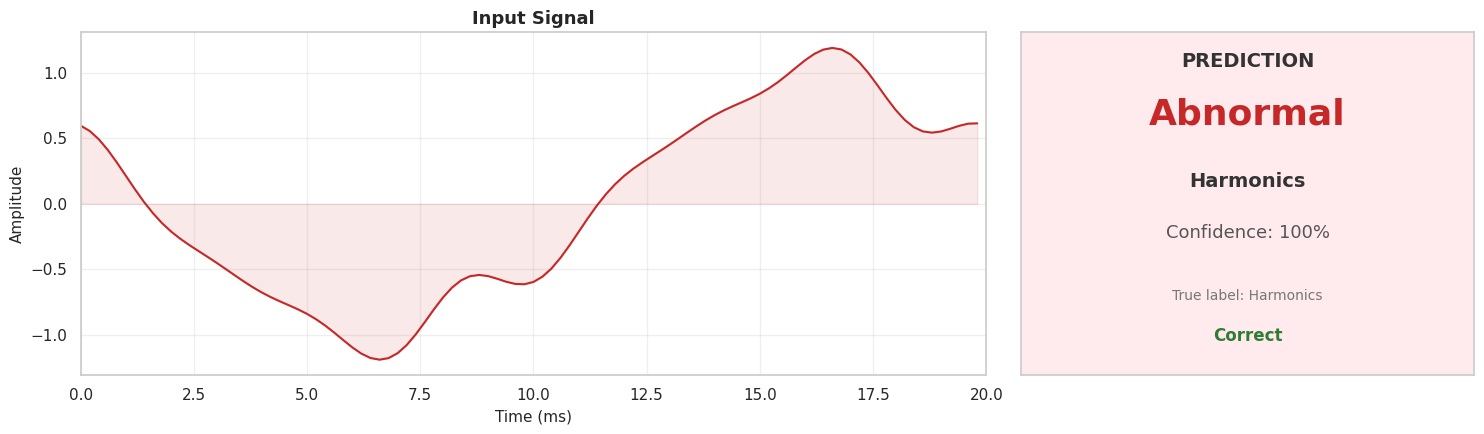
\includegraphics[width=0.75\linewidth]{image3.png}
    \caption{Sample prediction output illustrating input voltage waveform and corresponding classification result with disturbance type and confidence score}
    \label{fig:output}
\end{figure}
\begin{figure}[h]
    \centering
    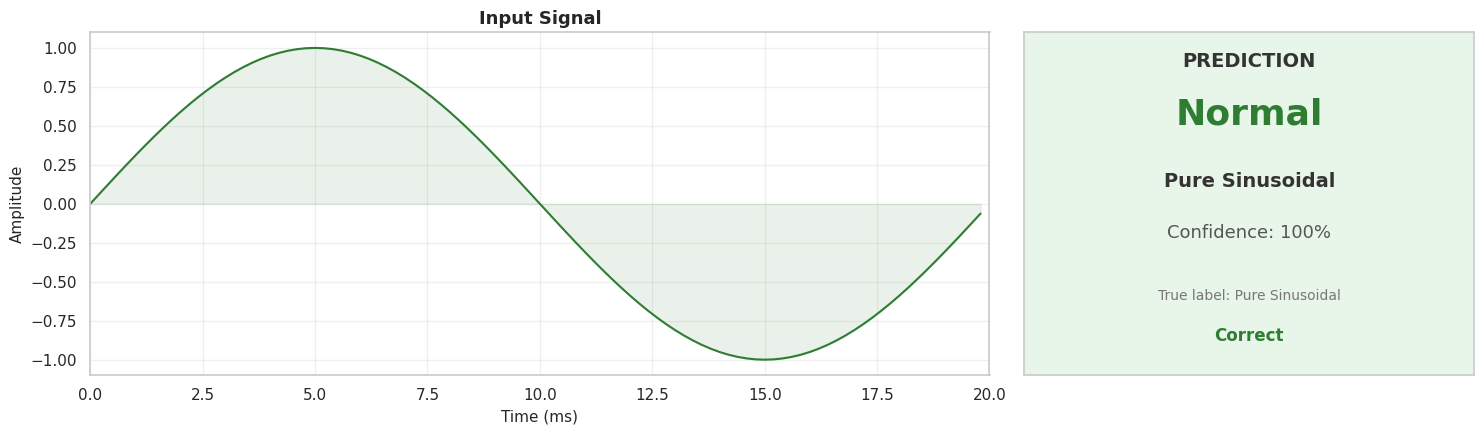
\includegraphics[width=0.75\linewidth]{image4.png}
    \caption{Sample prediction output for a normal operating condition showing pure sinusoidal waveform and correct classificationhttps://meet.google.com/ert-gmdy-sne with associated confidence level}
    \label{fig:normal_output}
\end{figure}

Fig.~\ref{fig:output} illustrates a representative output of the proposed system for an abnormal input signal.

In this case, the model identifies the signal as an abnormal condition corresponding to harmonic distortion with a confidence score of 100\%. The correct classification demonstrates the capability of the model to accurately capture disturbance characteristics.

Fig.~\ref{fig:normal_output} presents the model output for a normal operating condition. The system correctly classifies the signal as a normal waveform with high confidence, demonstrating its ability to distinguish between normal and disturbed signals effectively.

The visualization of both abnormal and normal cases highlights the interpretability of the system, where waveform characteristics and classification outputs are presented together. This supports practical deployment in real-time monitoring environments.

\subsection{Discussion}

The results demonstrate that the proposed framework effectively classifies power quality disturbances using multi-domain feature extraction and Random Forest classification. The optimized hyperparameters contribute to improved model stability and generalization.

The ensemble nature of Random Forest reduces variance and enhances robustness, enabling consistent performance across different datasets. The ability to correctly classify both abnormal and normal signals minimizes false alarms, which is critical in real-world power system applications.

Compared to deep learning approaches, the proposed method offers lower computational complexity and easier deployment while maintaining high classification accuracy. Additionally, the inclusion of confidence-based predictions improves the reliability and usability of the system.

Overall, the proposed approach achieves a balance between accuracy, interpretability, and computational efficiency, making it a suitable solution for real-time power quality disturbance monitoring.

\begin{thebibliography}{00}
\bibitem{b1} A. A. Memon, M. A. Koondhar, S. F. Al-Gahtani, Z. M. S. Elbarbary,
    and Z. M. Alaas, "Comprehensive review of power quality disturbance
    detection and classification techniques," Comput. Electr. Eng.,
    vol. 126, Aug. 2025.
\bibitem{b2}  S. Janthong and P. Phukpattaranont, "Power quality disturbance
    detection using improved grasshopper optimization and adaptive
    boosted random forest," Electr. Eng., Springer, 2025.
\bibitem{b3} S. Wei, D. Wenjuan, and C. Xia, "Power quality disturbances
    categorization using identity feature vector and extreme learning
    machine," Intell. Syst. Appl., vol. 24, p. 200446, 2024.
\bibitem{b4} P. M. Peruman and K. Ayyar, "Power quality disturbance
    identification using hybrid deep learning in renewable energy
    systems," Sci. Rep., vol. 15, 2025.
\bibitem{b5} S. S. Akkaya, E. Yuksek, and H. M. Akgun, "A comprehensive
    research of machine learning algorithms for power quality
    disturbances classifier based on time-series window,"
    Electr. Eng., vol. 106, pp. 3983-4001, 2024.
\bibitem{b6} R. J. J. Molu, W. F. Mbasso, K. T. Saatong, and S. R. D. Naoussi,
    "Enhancing power quality monitoring with discrete wavelet transform
    and extreme learning machine: a dual-stage pattern recognition
    approach," Front. Energy Res., vol. 12, p. 1435704, 2024.
\bibitem{b7} S. Jain, A. Satsangi, R. Kumar, and D. Panwar, "Intelligent
    assessment of power quality disturbances: a comprehensive review
    on machine learning and deep learning solutions," Comput. Electr.
    Eng., vol. 123, 2025.
\bibitem{b8} M. S. Priyadarshini, M. Bajaj, L. Prokop, and M. Berhanu, "Perception of power quality disturbances using Fourier, short-time Fourier, continuous and discrete wavelet transforms," Sci. Rep., vol. 14, p. 3443, Feb. 2024.
\bibitem{b9} M. S. Priyadarshini, M. Bajaj, and I. Zaitsev, "Energy feature extraction and visualization of voltage sags using wavelet packet analysis for enhanced power quality monitoring," Sci. Rep., vol. 15, p. 2226, Jan. 2025 .
\bibitem{b10}  M. H. Anwar, M. M. A. Baig, A. J. Shaikh, and A. G. Abro,
     "Detection and classification of power quality disturbances:
     vision transformers vs. CNN," AIMS Energy, vol. 13, no. 5,
     pp. 1052-1075, 2025.
\end{thebibliography}
\vspace{12pt}

\end{document}
